\documentclass[11pt]{article}
\usepackage{amsmath}
%\usepackage{extsizes}
\usepackage{amsmath,amssymb}
%\usepackage{omegavn,ocmrvn}
%\usepackage[utf8x]{inputenc}
\usepackage[utf8]{vietnam}

\usepackage{longtable}
\usepackage{answers}

\usepackage{graphicx}
\usepackage{float}

\usepackage{listings}
\lstset{language=Python}          % Set your language (you can change the language for each code-block optionally)

\usepackage{array}
\usepackage{pifont}
\usepackage{picinpar}
\usepackage{enumerate}
\usepackage[top=3.0cm, bottom=3.5cm, left=3.5cm, right=2.5cm] {geometry}
\usepackage{hyperref}


\newtheorem{bt}{Câu}
\newcommand{\RR}{\mathbb R}
\Newassociation{sol}{Solution}{ans}
\newtheorem{ex}{Câu}
\renewcommand{\solutionstyle}[1]{\textbf{ #1}.}
\newcommand{\m}[1]{\begin{bmatrix}
		#1
\end{bmatrix}}

\begin{document}
% \noindent
\begin{tabular*}
{\linewidth}{c>{\centering\hspace{0pt}} p{.7\textwidth}}
Trường ĐHKHTN, ĐHQGHN & {\bf Học Kỳ 1 (2019-2020)}
\tabularnewline
K63 TTƯD - Thầy Hà Phi & {\bf Bài Tập Giải Tích Số. No 6 \\ Giải hệ pt tuyến tính Ax=b}
% Exercises on pages 239, 240 Cheney/Kincaid are really nice
\tabularnewline
\rule{1in}{1pt}  \small  & \rule{2in}{1pt} %(Due date:)
\tabularnewline

%  \tabularnewline
%  &(Đề thi có 1 trang)
\end{tabular*}
%
% \Opensolutionfile{ans}[ans1]
\vskip .2cm

Tìm hiểu toolbox linalg trong Python \url{https://docs.scipy.org/doc/numpy-1.15.1/reference/routines.linalg.html}.

\begin{bt}
Bốn vật nặng có khối lượng khác nhau $m_i$ được nối với nhau bằng những sợi dây có khối lượng không đáng kể. Ba trong số các khối nằm trên một mặt phẳng nghiêng, hệ số ma sát giữa các khối và mặt phẳng là $\mu_i$. Phương trình chuyển động của các khối có thể được biểu diễn là
%
\begin{align*}
T_1 + m_1a &= m_1g (\sin \theta - \mu_1 \cos \theta) \\
-T_1 + T_2 + m_2a &= m_2g (\sin \theta - \mu_2 \cos \theta) \\
-T_2 + T_3 + m_3a &= m_3g (\sin \theta - \mu_3 \cos \theta) \\
-T_3 + m_4a &= -m_4 g .
\end{align*}
%
Trong đó $T_i$ biểu thị lực kéo trong các sợi dây và $a$ là gia tốc của
hệ thống. Xác định $a$ và $T_i$ nếu $\theta = 45^o$, $g = 9,82 m / s^2$ và
$m = \m{10 & 4 & 5 & 6}^T$ kg, $\mu = \m{0.25 & 0.3 & 0.2}^T$.
%	
\begin{figure}[h!]
	\centering
	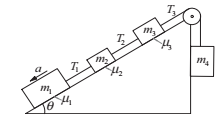
\includegraphics[width=0.4\linewidth]{mass_rope}
	\caption[]{Exercise 25, page 58, Kiusalass}
	\label{fig:massrope}
\end{figure}

\end{bt}

\begin{bt}
Công thức chuyển dời của hệ lò xo khối lượng được chỉ ra trong Hình (a) dẫn đến các phương trình cân bằng sau của các khối lượng
%
\[
\m{	k_1 + k_2 + k_3 + k_5 & -k_3 & -k_5 \\
	-k_3 & k_3 + k_4 & -k_4 \\
	-k_5 & -k_4 & k_4 + k_5
}
\m{	x_1 \\
	x_2 \\
	x_3
}
=
\m{ W_1 \\ W_2 \\ W_3}
\]
%
trong đó $k_i$ là độ cứng của lò xo, $W_i$ đại diện cho trọng lượng của các khối lượng và $x_i$ là độ dịch chuyển của các khối lượng từ cấu hình không định dạng của hệ thống. Viết chương trình giải các phương trình này cho k và W là các đầu vào, còn x là đầu ra. 
Sử dụng chương trình để tìm các chuyển vị nếu
\begin{align*}
k_1 &= k_3 = k_4 = k, \ k_2 = k_5 = 2k, \\
W_1 &= W_3 = 2W, \ W_2 = W \ .
\end{align*}

\begin{figure}[h!]
	\centering
	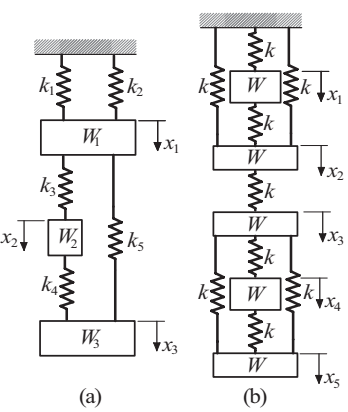
\includegraphics[width=0.3\linewidth]{mass_spring}
	\caption{Exercise 12, page 79, Kiusalass}
	\label{fig:massspring}
\end{figure}
\end{bt}

\begin{bt}
Công thức chuyển dời của giàn phẳng tương tự như công thức của hệ lò xo khối lượng. Sự khác biệt là (1) độ cứng của các bộ phận là $k_i = (EA / L)_i$, trong đó E là mô đun đàn hồi, A đại diện cho diện tích mặt cắt ngang, và L là chiều dài của bộ phận; và (2) có hai thành phần chuyển vị tại mỗi khớp. Đối với giàn không xác định tĩnh được hiển thị, công thức chuyển vị cho ra phương trình đối xứng $Ku = p$, trong đó
\begin{align*}
K &=
\m{	27.58 & 7.004 &-7.004 &0 &0 \\
	7.004 &29.57& -5.253& 0 &-24.32 \\
	-7.004 &-5.253 &29.57& 0& 0 \\
	0& 0& 0& 27.58& -7.004 \\
	0& -24.32& 0 &-7.004& 29.57} \quad MN/m \ (\mbox{millinewton/metre}) \\
p &= \m{0 &0& 0& 0& -45}^T \quad kN \ (\mbox{kilonewton}) \ .
\end{align*}
Xác định các vị trí $u_i$ của các khớp.

\begin{figure}[h!]
	\centering
	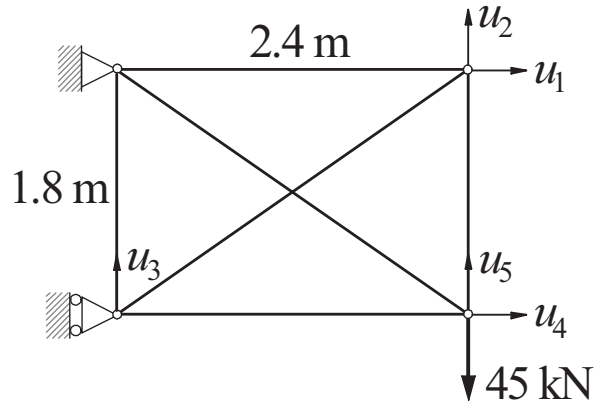
\includegraphics[width=0.5\linewidth]{plane_truss}
	\caption{Exercise 14, page 79, Kiusalass}
	\label{fig:planetruss}
\end{figure}
\end{bt}


\begin{bt}
Bốn thùng trộn được nối với nhau bằng đường ống. Chất lỏng trong hệ thống được bơm thông qua các đường ống với tỷ lệ hiển thị trong hình. Chất lỏng vào hệ thống
chứa hóa chất có nồng độ c theo chỉ định. Xác định nồng độ của hóa chất trong bốn bình, giả sử ở trạng thái dừng.
\begin{figure}[h!]
	\centering
	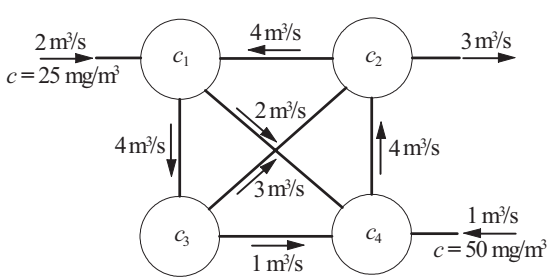
\includegraphics[width=0.5\linewidth]{mixing_tank}
	\caption{}
	\label{fig:mixingtank}
\end{figure}
\end{bt}

\begin{bt} Viết hàm Python để tìm phân tích LU. Từ đó sử dụng phương pháp Gauss để giải hệ phương trình sau
%
\begin{align*}
 2 x_1 + 4 x_2 + 3x_3   &= 3, \\
 3 x_1 + x_2 - 2 x_3    &= 3, \\
 4 x_1 + 11 x_2 + 7 x_3 &= 4. 
\end{align*}
%
So sánh kết quả của các em với cách giải sử dụng toolbox linalg trong Python. 
\end{bt}

\begin{bt} Giả sử ma trận $A$ thỏa mãn $PA = LU$, trong đó
\begin{figure}[h!]
	\centering
	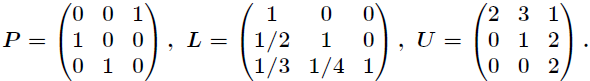
\includegraphics[scale = 0.7]{3}
\end{figure}
a) Hãy sử dụng các ma trận trên để giải hệ phương trình $Ax=b$ với $b = \m{2 & 10 & -12}^T$ mà không cần tìm ma trận $A$ hay tìm nghich đảo của $A$.
b, Có thể nhận thấy ma trận P nhận được từ ma trận đơn vị bằng cách hoán vị các hàng. Hãy nêu ý nghĩa của việc nhân một ma trận với $P$ từ bên trái.
\end{bt}

\centering{------------------------------Kết thúc phần 1--------------------------------------}

\newpage 
\begin{bt}
Trong trường hợp ma trận A là đối xứng, xác định dương thì phương pháp Cholesky thường được sử dụng. Hãy đọc phương pháp này trang 116-120 (Giáo trình ĐHBK) hoặc Section 2.4 (Giáo trình Kiusalass) và tìm hiểu hàm $numpy.linalg.cholesky$ trong Python. Áp dụng để giải hệ phương trình sau đối với vế phải $b$ lần lượt bằng $[2 \ 3 \ 0]^T$ và $[2 \ 5 \ -2]^T$.
	%
	\begin{align*}
	4 x_1 - 2 x_2 + 4 x_3   &= b_1, \\
	-2 x_1 + 5 x_2 - 4 x_3  &= b_2, \\
	4 x_1  -4 x_2 + 6 x_3   &= b_3. 
	\end{align*}
	%
\end{bt}

\begin{bt}
\end{bt}

\begin{center}
  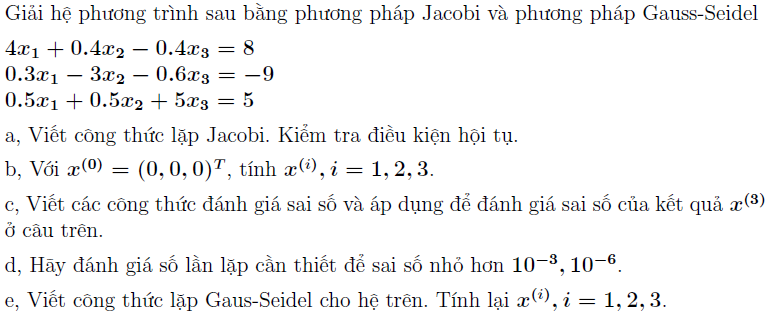
\includegraphics[scale = 0.7]{4}	
\end{center}

\begin{bt}
\end{bt}
\begin{figure}[H]
	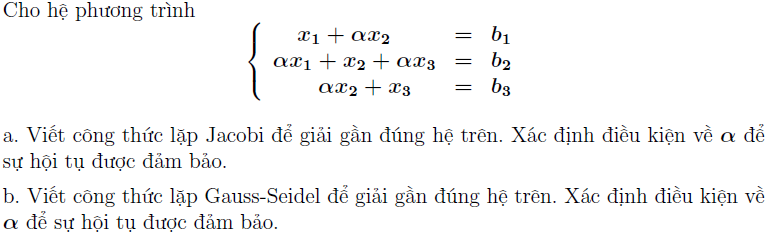
\includegraphics[scale = 0.7]{5}
\end{figure}
c. Từ các tính toán ở hai câu trên, hãy so sánh tốc độ hội tụ của hai phương pháp.

\vskip .5cm

\centerline{———————————Hết——————————-}

\end{document}

\vspace{1cm}
\noindent{\bf Chú ý:} {\it Cán bộ coi thi không giải thích gì thêm}\\
\Closesolutionfile{ans}
\newpage
\begin{center}
{\LARGE{\bf ĐÁP ÁN}}
\end{center}

\begin{sol}
	\begin{figure}[h!]
		\centering
		\includegraphics[width=0.8\linewidth]{Solution1/Sol4_1.png}
		%\caption{}
		\label{fig:Sol4}
	\end{figure}
	Exercise 7: Convergence order is 3.	
\end{sol}

   
\end{document}



